\documentclass[11pt, letterpaper, UTF-8]{article}
\usepackage{geometry}
\geometry{top=1in}
\usepackage{verbatim}      
\usepackage{lipsum}           		
\usepackage{graphicx}
\usepackage{amssymb}
\usepackage{tabularx}
\usepackage[utf8]{inputenc}
\usepackage{array}
\usepackage[english]{babel}
\usepackage{graphicx}
\usepackage{indentfirst}

\pagestyle{empty}

\title{}
\author{}
\date{\textsc{\today}}
\begin{document}

\begin{center}
{\huge \textsc{Keyboard Shortcuts for Twitch}}
\bigskip\\
{\Large \textsc{Hudson Duan}}\\
\today\\
\end{center}
\section{Overview}
Twitch is a live streaming service, initially focused on gaming but recently expanding into providing artists and other creatives a place to stream their work to a broad audience. The service was acquired by Amazon last year for almost a billion dollars in cash and is at the forefront of the eSports movement. Streams can often last multiple hours and seeking to a specific timestamp on a saved video is very difficult without \textit{keyboard commands}.

\section{Proposal}

\indent\begin{tabular}{r|p{14cm}}

\textsc{Problem} & Twitch saves streams so that people who missed the live broadcast can watch them later. However, the timescale of live broadcasts are often magnitudes larger than uploaded content on similar websites such as Youtube, and using a mouse to seek to a specific timestamp is often impractical or even impossible. For example, 24-hour streams are commonplace on Twitch, and if somebody wants to watch a highlight starting at exactly 8:24:35, the seek bar on the HTML5 player does not give enough precision.\\
\\
\textsc{Solution} & Keyboard commands entered via a command line interface eliminate this disconnect between user input device and precision required. By inserting a small text input box (Figure 1) in the empty space between the volume control and full-screen button, a user has access to a series of commands that allow seeking to specific timestamps and seeking by elapsed time such as rewinding or fast-forwarding by 30s. Once users adopt the command line interface, collapsing the volume controls, video quality select, and other options entirely into commands is also a possibility.\\

\end{tabular}



\section{User Profile}
Twitch is a relatively new service and caters to a very specific set of users, young adult gamers. Ages typically range between early teens to late twenties, and competence with computers can be assumed to be high. Along with sites such as reddit, users of Twitch strongly identify with internet culture.\\

\begin{center}
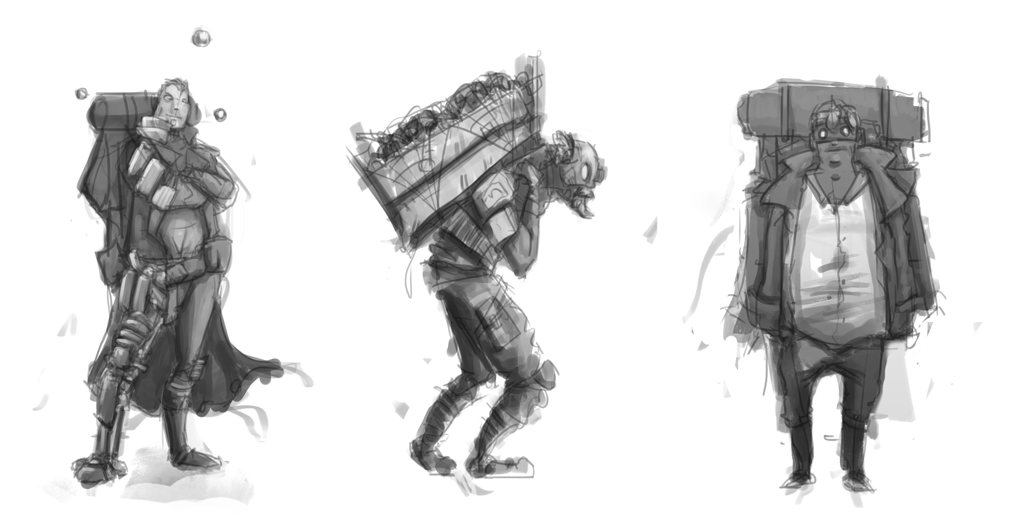
\includegraphics[width=0.4\textwidth]{gamer.png}
\end{center}
\newpage
Our assumption is that Twitch users are computer power-users and thus necessitates power-user behavior. Taking a page from Photoshop and Vim pros, keyboard commands drastically reduce the time it takes for repetitive tasks, as well as embedding users in a familiar computing paradigm. Our proposal identifies Twitch's hardcore gamer user-base and molds a solution accordingly.\\
\section{Implementation}
Twitch has a custom built HTML5 video player thus inserting an input box to send javascript commands is relatively trivial. Edge cases to consider are various browser resizing issues and mobile. A staggered rollout of this feature is recommended, targeting Twitch users that spend the most time on the service and the users that have paid the most through the donation system as this isolates the most passionate of users. Gather feedback, iterate appropriately and extend the functionality to more users over time.\\

\section{Marketing}
Since this is a relatively small feature, overt marketing can be kept at a minimum and concentrate on customer support if there are questions or a backlash. Comparisons can be drawn to Youtube offering small thumbnail previews while seeking as opposed to large media campaigns for YoutubeRed or Vevo. If feedback is quiet, request surveys and monitor usage data of the keyboard commands vs manual mouse seeks through request payload data.\\

\section{Conclusion}
Keyboard commands are a natural progression of user input as videos grow larger and users spend more time watching them. Twitch can benefit from implementing a command line interface as there is empty space in their custom video player and catering to a userbase of hardcore gamers. I hope this exercise gives a glimpse of my skills as a product manager as well as showing that I still have much to learn from the best in the industry. Thanks for your consideration. \\

\newpage
\begin{figure}[p]
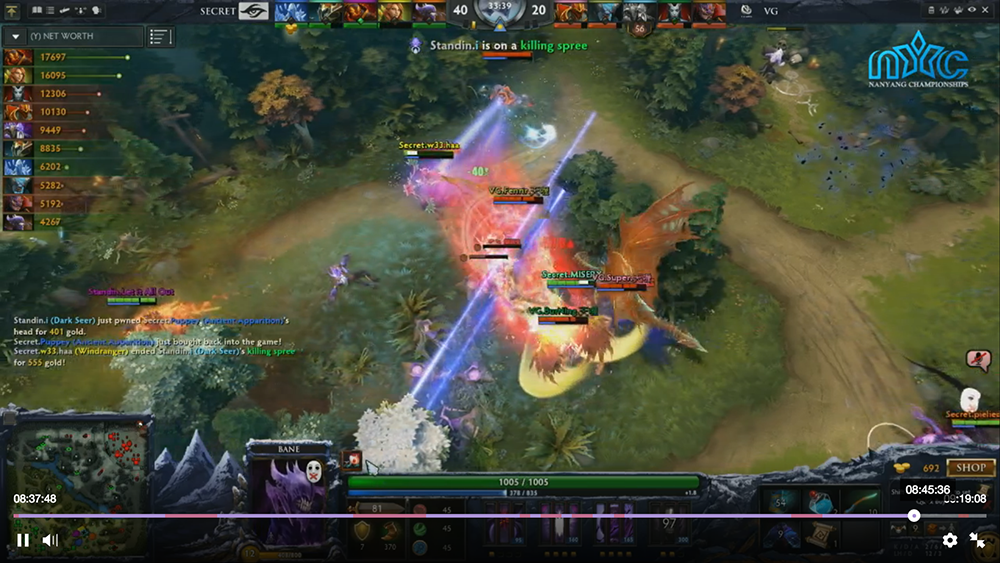
\includegraphics[width=1\textwidth]{twitchnoblur}
\\\smallskip\\
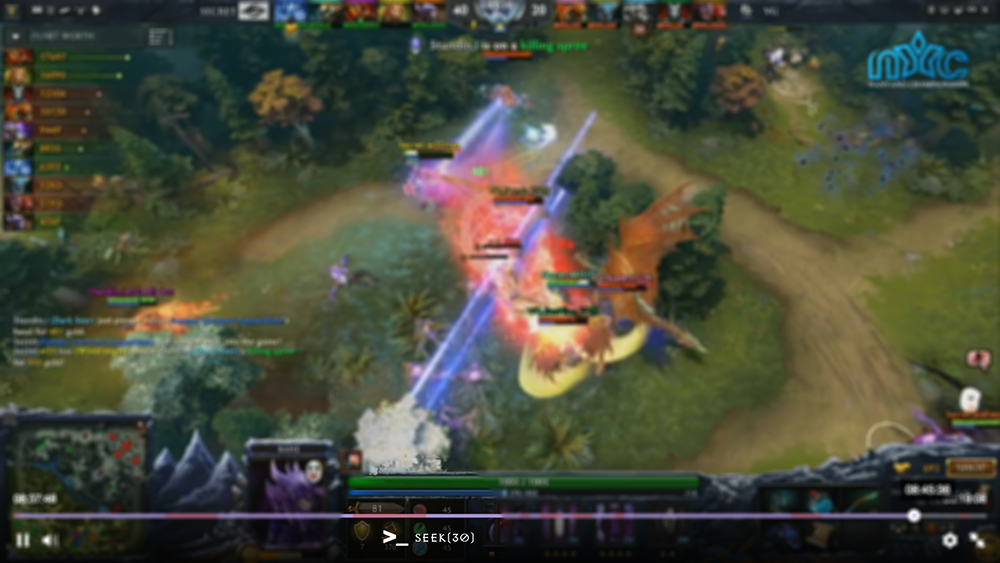
\includegraphics[width=1\textwidth]{twitch}
\caption{Command line interface proposal (See video length of over 9hrs)}
\end{figure}

\end{document} 